\onecolumn

\section{Experiment Details} \label{apdx: expdetails}

We conduct our experiments on several variants of two models: LLaDA-8B-Instruct \cite{llada}, LLaDA-1.5 \cite{llada1.5}, Dream-v0-Base-7B \cite{dream}, Dream-v0-Instruct-7B. Benchmarks include diverse datasets: GSM8K (5-shot) \cite{gsm8k}, MATH (4-shot) \cite{math}, HumanEval (0-shot) \cite{humaneval}, and MBPP (3-shot) \cite{mbpp}, covering a range of reasoning and code generation tasks. Across all settings, we fix the block size to 32 and generation length to 256 tokens except KLASS, which uses its best-performing block length.

All baselines are evaluated under their default hyperparameter settings. To identify the optimal hyperparameter configuration for our method \dawn{} on different models, including $\tau_{edge}$, $\tau_{induced}$ and $\tau_{sink}$, we conduct a grid search on the HumanEval dataset. Specifically, we evaluate a range of candidate values for each parameter and plot the corresponding Accuracy–TPS curves, visualized in Fig~\ref{fig:llada-8b-instruct}, \ref{fig:llada-1.5}, \ref{fig:dream-base}, \ref{fig:dream-instruct}.

\begin{figure}[htbp]
    \centering
    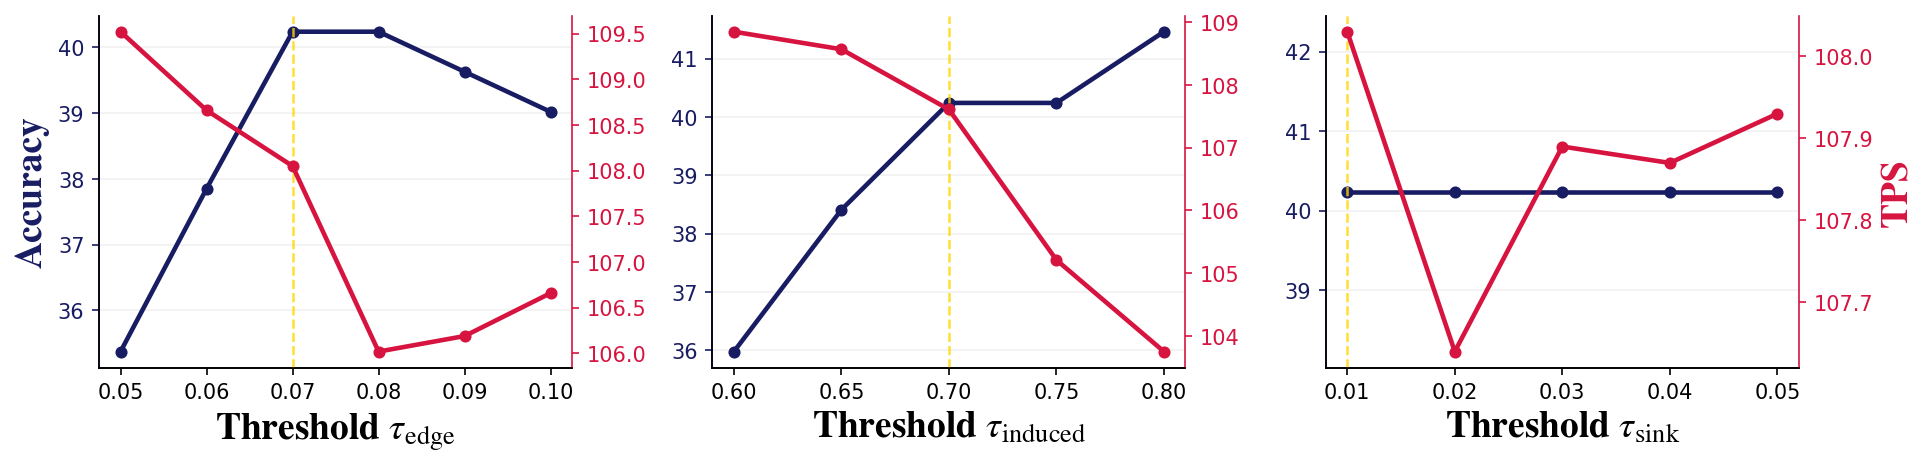
\includegraphics[width=\linewidth]{fig/LLaDA-8B-Instruct.png}
    \caption{\textbf{We vary the threshold $\tau_{edge}$, $\tau_{induced}$, $\tau_{sink}$ and report accuracy (blue, left y-axis) and throughput TPS (red, right y-axis) on LLaDA-8B-Instruct}. The dashed lines (yellow) mark the final settings $\tau_{edge}$ = 0.07, $\tau_{induced}$ = 0.70, $\tau_{sink}$ = 0.01.}
    \label{fig:llada-8b-instruct}
\end{figure}

\begin{figure}[htbp]
    \centering
    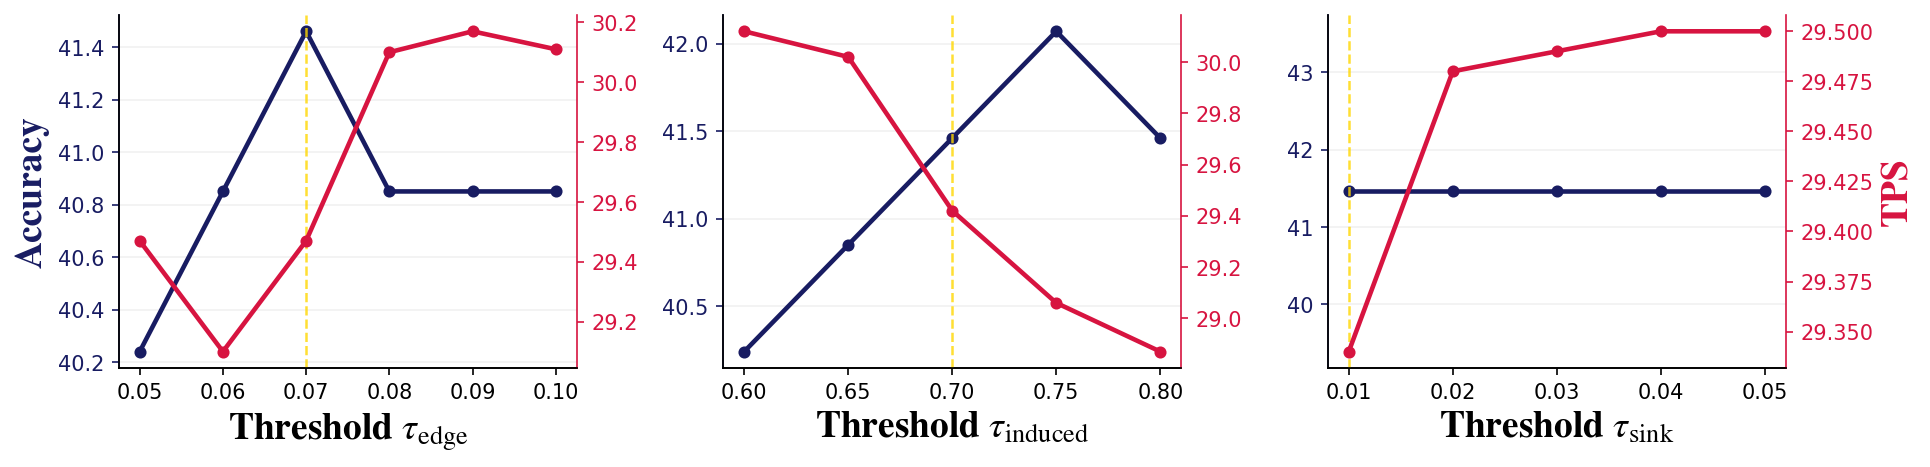
\includegraphics[width=\linewidth]{fig/LLaDA-1.5.png}
    \caption{\textbf{We vary the threshold $\tau_{edge}$, $\tau_{induced}$, $\tau_{sink}$ and report accuracy (blue, left y-axis) and throughput TPS (red, right y-axis) on LLaDA-1.5}. The dashed lines (yellow) mark the final settings $\tau_{edge}$ = 0.07, $\tau_{induced}$ = 0.70, $\tau_{sink}$ = 0.01.}
    \label{fig:llada-1.5}
\end{figure}

\begin{figure}[htbp]
    \centering
    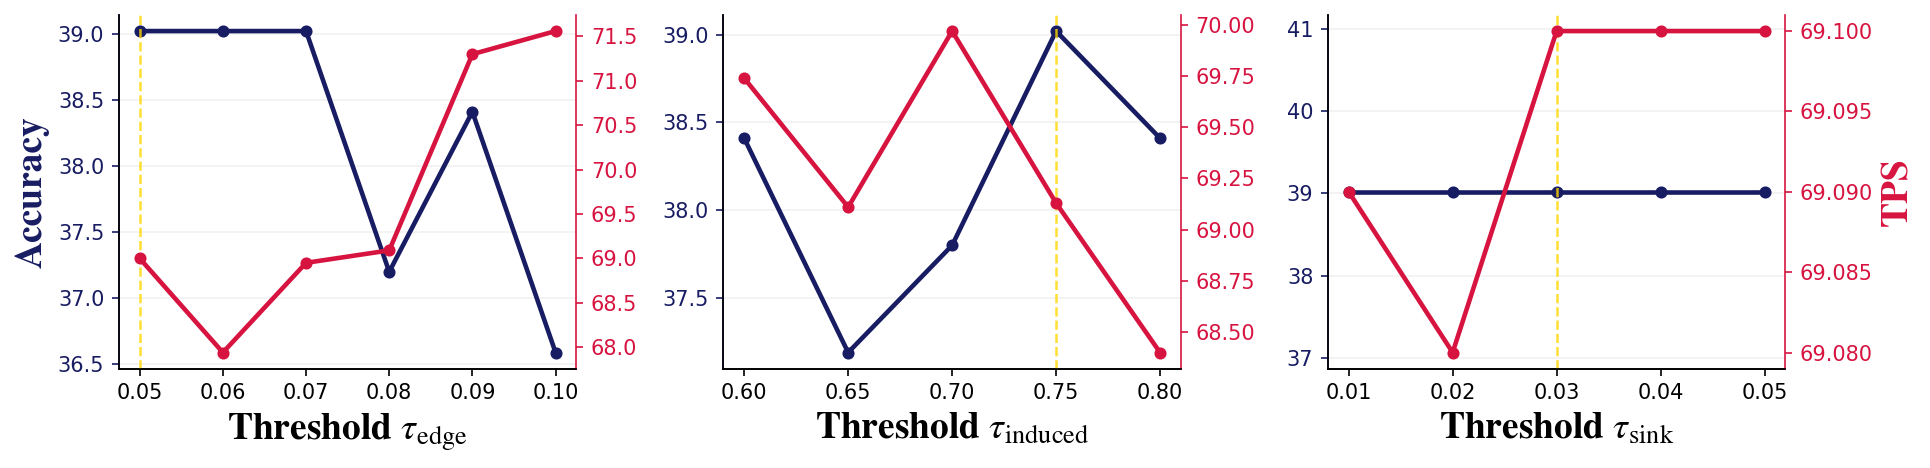
\includegraphics[width=\linewidth]{fig/Dream-v0-Base-7B.png}
    \caption{\textbf{We vary the threshold $\tau_{edge}$, $\tau_{induced}$, $\tau_{sink}$ and report accuracy (blue, left y-axis) and throughput TPS (red, right y-axis) on Dream-v0-Base-7B}. The dashed lines (yellow) mark the final settings $\tau_{edge}$ = 0.05, $\tau_{induced}$ = 0.75, $\tau_{sink}$ = 0.03.}
    \label{fig:dream-base}
\end{figure}

\begin{figure}[h!]
    \centering
    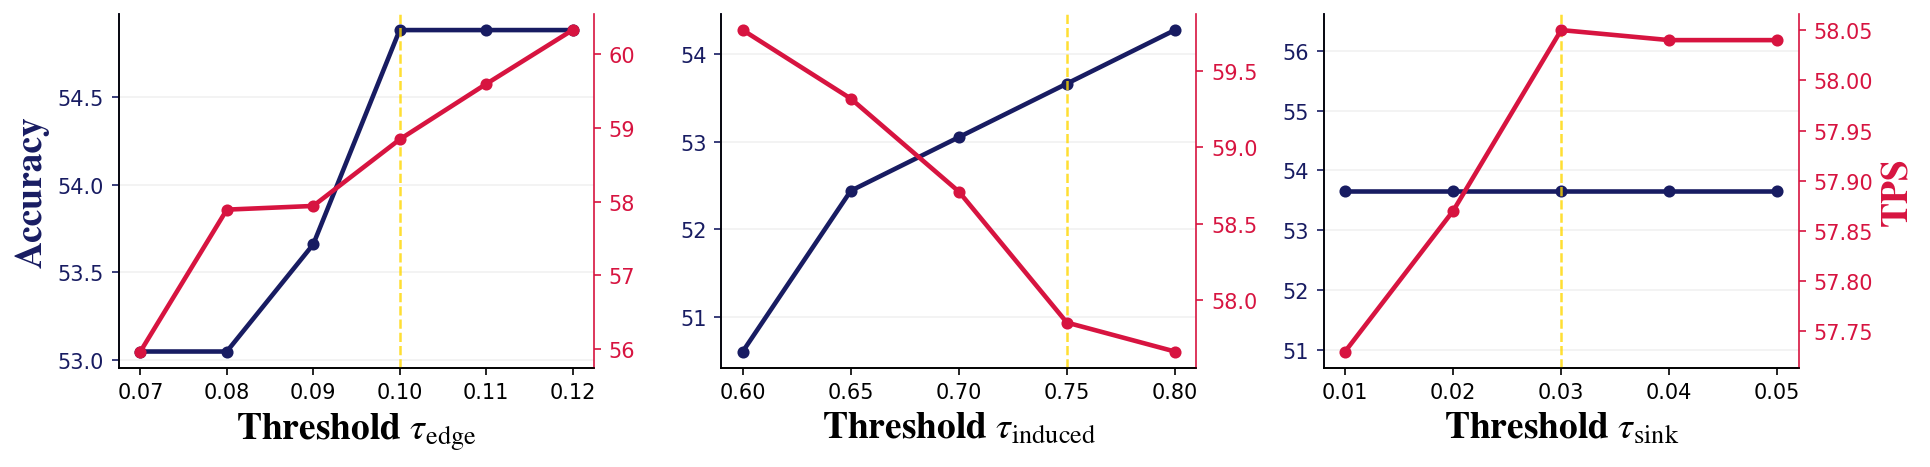
\includegraphics[width=\linewidth]{fig/Dream-v0-Instruct-7B.png}
    \caption{\textbf{We vary the threshold $\tau_{edge}$, $\tau_{induced}$, $\tau_{sink}$ and report accuracy (blue, left y-axis) and throughput TPS (red, right y-axis) on Dream-v0-Instruct-7B}. The dashed lines (yellow) mark the final settings $\tau_{edge}$ = 0.10, $\tau_{induced}$ = 0.75, $\tau_{sink}$ = 0.03.}
    \label{fig:dream-instruct}
\end{figure}

In most cases, we observe a clear trade-off between throughput and accuracy: higher throughput is generally achieved at the cost of reduced accuracy. To balance this trade-off, we select hyperparameter values that lie near the Pareto frontier, favoring configurations that preserve high accuracy while providing meaningful efficiency gains. For example, on the LLaDA-8B-Instruct model, we select $\tau_{edge} = 0.07$, which achieves the highest accuracy among the tested values while offering higher throughput compared to $\tau_{edge} = 0.08$. This criterion ensures that the chosen configuration does not sacrifice accuracy for marginal speed improvements.

For the \textit{the lower confidence threshold $\tau_{low}$} hyperparameter, we perform a grid search over both models and benchmarks, resulting in 16 experimental settings in total. Within each setting, we further tune the method-specific hyperparameters to obtain the best-performing configuration. The final selected results are reported in Table~\ref{tab:4x4}.

% \begin{table}[t!]
%   \centering
%   \begin{tabular}{*{8}{c}}
%     \toprule
%     & \multirow{2}{*}{$\tau_{edge}$} & \multirow{2}{*}{$\tau_{induced}$} & \multirow{2}{*}{$\tau_{sink}$} & \multicolumn{4}{c}{Confidence} \\
%     \cmidrule{5-8}
%     Model & & & & GSM8K & MATH & HumanEval & MBPP \\
%     \midrule
%     LLaDA-8B-Instruct & 0.01 & 0.07 & 0.70 & XX & XX & XX & XX\\
%     LLaDA-1.5 & 0.01 & 0.07 & 0.70 & XX & XX & XX & XX\\
%     Dream-v0-Base-7B & 0.03 & 0.05 & 0.75 & XX & XX & XX & XX\\
%     Dream-v0-Instruct-7B & 0.03 & 0.10 & 0.75 & XX & XX & XX & XX\\
%     \bottomrule
%     \end{tabular}
%   \caption{A 4×4 Table with Row and Column Labels}
%   \label{tab:4x4}
% \end{table}

\begin{table}[htbp]
  \centering
  \caption{\textbf{Final hyperparameter settings for \dawn{}, where rows denote models and columns denote hyperparameter types}. The $\tau_{induced}$, $\tau_{sink}$, $\tau_{edge}$ are shared across benchmarks for each model, while $\tau_{low}$ adopt benchmark-specific configurations.}
  \begin{tabular}{*{8}{c}}
    \toprule
    & \multirow{2}{*}{\textbf{$\tau_{induced}$}} & \multirow{2}{*}{\textbf{$\tau_{sink}$}} & \multirow{2}{*}{\textbf{$\tau_{edge}$}} & \multicolumn{4}{c}{$\tau_{low}$} \\
    \cmidrule{5-8}
    Model & & & & GSM8K & MATH & HumanEval & MBPP \\
    \midrule
    LLaDA-8B-Instruct     & 0.70 & 0.01 & 0.07 & 0.75 & 0.75 & 0.8 & 0.7\\
    LLaDA-1.5             & 0.70 & 0.01 & 0.07 & 0.75 & 0.75 & 0.8 & 0.75\\
    Dream-v0-Base-7B       & 0.75 & 0.03 & 0.05 & 0.75 & 0.8 & 0.8 & 0.8\\
    Dream-v0-Instruct-7B   & 0.75 & 0.03 & 0.10 & 0.8 & 0.8 & 0.8 & 0.8\\
    \bottomrule
  \end{tabular}
  \label{tab:4x4}
\end{table}

\section{Discussion}
This work is primarily motivated by the challenge of nonindependent position predictions in dLLMs, which suggests that decoding order should account for dependencies among positions. In many existing analyses and methods, high confidence is often treated as a sufficient indicator of per-position consistency or approximate independence, and the resulting update rules largely rely on such conservative criteria, which can limit achievable parallelism and leave a substantial portion of dLLM parallel potential underexploited. In contrast, this work attempts to capture positional coupling more directly and to derive corresponding decoding strategies from these dependency relations.

Viewing dLLM decoding through the lens of positional dependencies provides a complementary perspective that can more directly address the persistent difficulty of parallel decoding under non-independence. It is hoped that this study will encourage further investigation into dependency structures in dLLMs and inspire more efficient inference methods that leverage them.
